\documentclass{oblivoir}
\usepackage{amsmath,amssymb,amsthm,kotex,mdframed,paralist,kswrapfig}

\newcounter{num}
\newcommand{\prob}
{\bigskip\noindent\refstepcounter{num}\textbf{문제 \arabic{num})}\par}

\newcommand{\subprob}
{\bigskip\noindent\textbf{추가문제 \arabic{num}-1)}\par}

\newcommand{\subprobb}
{\bigskip\noindent\textbf{추가문제 \arabic{num}-2)}\par}

\newcommand{\ans}{{\raggedleft\textbf{답 : (\qquad\qquad\qquad\qquad\qquad\qquad)}
\par}\bigskip\bigskip}


\newcommand\ga{\text{(가)}}
\renewcommand\na{\text{(나)}}


%%%
\begin{document}
\Large

\title{승재 17 - 6학년 2학기 - 10}
\author{}
\date{\today}
\maketitle
%\tableofcontents

\newpage


%
\prob
다음 그림과 같이 A, B 두 개의 원기둥이 있습니다.
1m를 굴러가는데 A는 20바퀴 회전하였고 B는 15바퀴 회전했습니다.
A, B의 밑면의 반지름의 비를 구하세요.

\begin{figure}[h!]
\centering
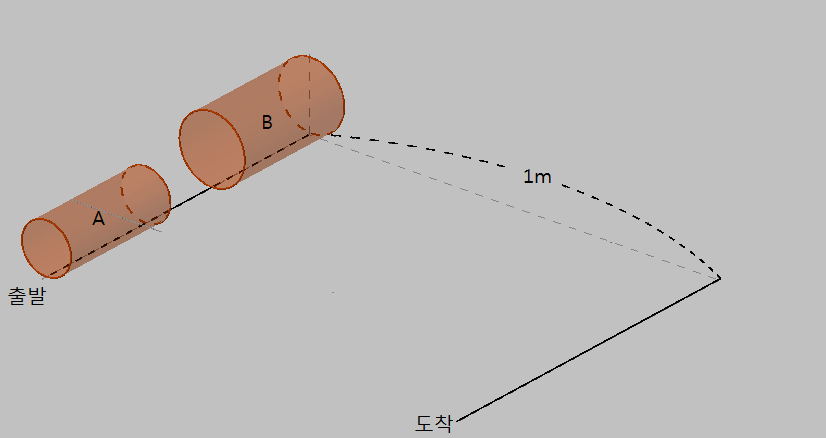
\includegraphics[width=0.7\textwidth]{01}
\end{figure}

\begin{mdframed}
\textbf{풀이 : }
\vspace{0.2\textheight}
\end{mdframed}
\ans

\newpage

%
\prob
다음 그림과 같이 A, B 두 개의 원기둥이 있습니다.
1m를 굴러가는데 A는 12바퀴 회전하였고 B는 16바퀴 회전했습니다.
A, B의 밑면의 넓이의 비를 구하세요.

\begin{figure}[h!]
\centering
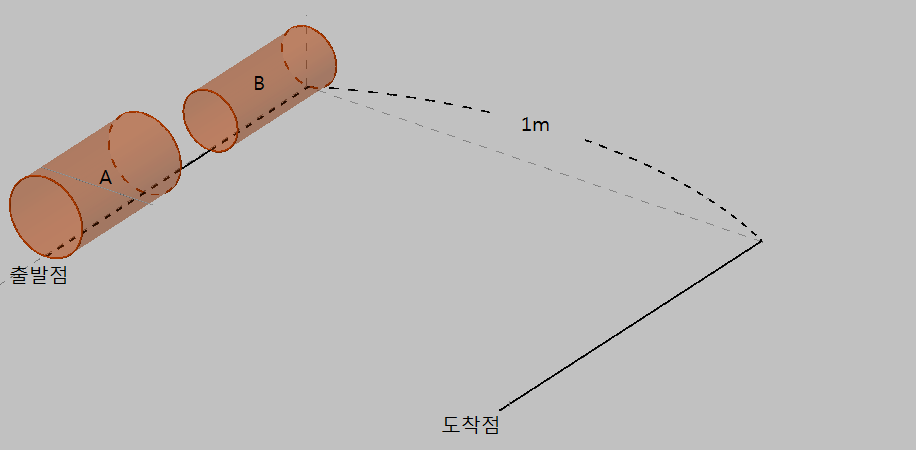
\includegraphics[width=0.7\textwidth]{02}
\end{figure}

\begin{mdframed}
\textbf{풀이 : }
\vspace{0.2\textheight}
\end{mdframed}
\ans

\newpage

%
\prob
다음 그림과 같이 밑면의 반지름의 길이와 높이가 같은 두 개의 원기둥 A, B가 있습니다.
두 원기둥에는 물감이 칠해져 있어서 굴러간 영역은 물감이 칠해집니다.
A가 15바퀴 회전하였고 B는 10바퀴 회전했을 때, A와 B의 바닥에 색칠된 영역의 넓이의 비를 구하세요.


\begin{figure}[h!]
\centering
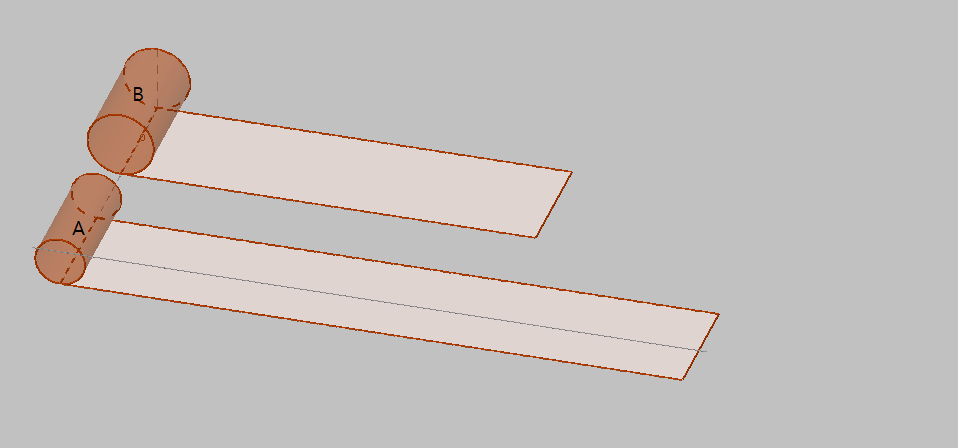
\includegraphics[width=0.7\textwidth]{03}
\end{figure}

\begin{mdframed}
\textbf{풀이 : }
\vspace{0.2\textheight}
\end{mdframed}
\ans
%
%\prob
%다음 그림과 같이 두 개의 원기둥 A, B가 있습니다.
%원기둥 A의 반지름의 길이는 원기둥 B의 반지름의 길이의 두 배이고 높이는 서로 같습니다.
%두 원기둥에는 물감이 칠해져 있어서 굴러간 영역은 물감이 칠해집니다.
%두 원기둥이 같은 횟수만큼 회전했을 때, A와 B의 바닥에 색칠된 영역의 넓이의 비를 구하세요.
%
%\ans
\newpage

%
\prob
선분 AB와 선분 BD의 길이의 비는 1:2이고 선분 AC와 선분 CD의 길이는 서로 같습니다.
\begin{figure}[h!]
\centering
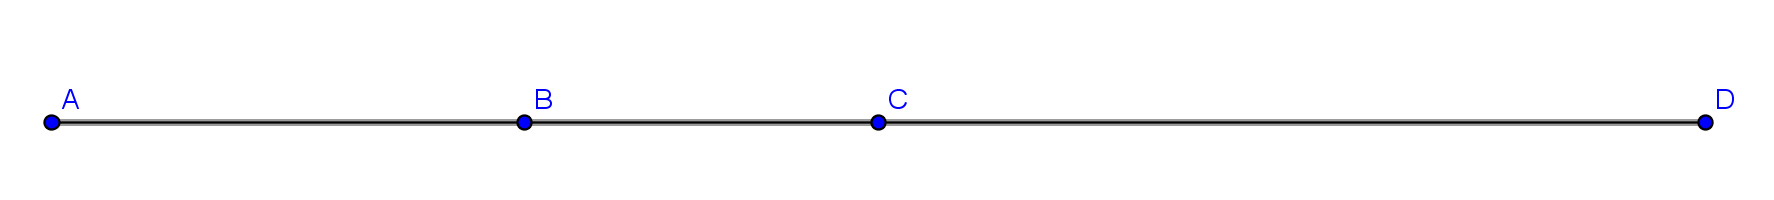
\includegraphics[width=0.9\textwidth]{04}
\end{figure}

이때, 선분 AB, 선분 BC, 선분 CD의 길이의 비를 구하세요.

\ans

%
\prob
선분 AB와 선분 BD의 길이의 비는 2:7이고 선분 AC와 선분 CD의 길이의 비는 4:1입니다.
\begin{figure}[h!]
\centering
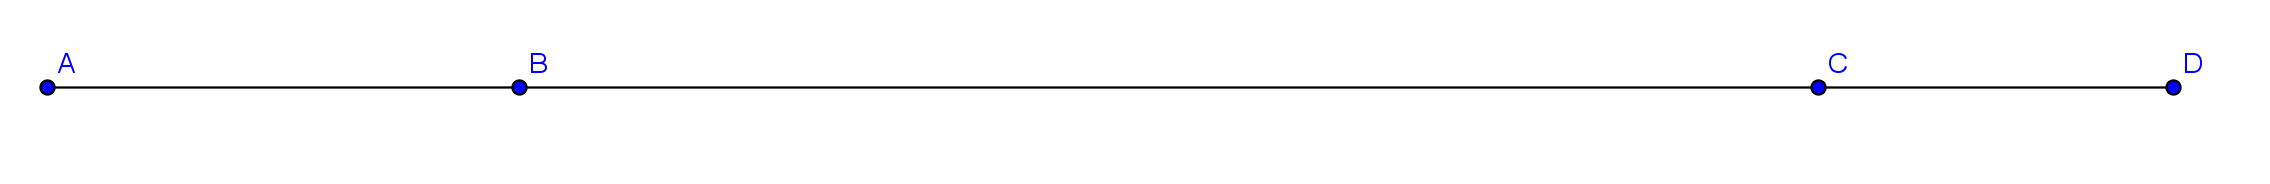
\includegraphics[width=0.9\textwidth]{05}
\end{figure}

이때, 선분 AB, 선분 BC, 선분 CD의 길이의 비를 구하세요.

\ans

\newpage


%
\prob
다음 \(\square\)에 들어갈 알맞은 숫자를 쓰세요.

\begin{enumerate}[(1)]
\item
\(3:1=\square:\frac37\)
\item
\(3:\frac35=8:\square\)
\item
\(\frac43:\frac32=2:\square\)
\item
\(\frac12:2=3:\square\)
\item
\(1:\frac73=\frac34:\square\)
\item
\(\frac35:\frac45=\square:10\)
\item
\(\frac{12}3:\frac{16}2=\square:\frac{25}2\)
\item
\(\frac{10}7:\frac{25}{11}=\square:28\)
\item
\(\frac{11}2:132=\square:2\)
\item
\(\frac{12}7:5=\frac{6}7:\square\)
\item
\(1.44:1.32=\square:33\)
\item
\(400:650=16:\square\)
\item
\(135:625=0.9:\square\)
\end{enumerate}

\newpage


%
\prob
준호가 이번 시험에서 받은 국어, 영어, 수학 점수를 살펴보았더니, 국어 점수는 영어 점수의 \(\frac67\)이고 수학 점수는 국어 점수의 \(\frac65\)이었습니다.
이 때, 수학 점수:영어 점수를 가장 간단한 자연수의 비로 나타내고, 그 풀이과정을 쓰세요.

\begin{mdframed}
\textbf{풀이 : }
\vspace{0.2\textheight}
\end{mdframed}
\ans

%
\prob
상재의 영어 점수는 국어 점수의 1.125이고 수학 점수는 영어 점수의 1.5입니다.
이 때, 수학 점수:국어 점수를 가장 간단한 자연수의 비로 나타내고, 그 풀이과정을 쓰세요.

\begin{mdframed}
\textbf{풀이 : }
\vspace{0.2\textheight}
\end{mdframed}
\ans

\newpage

%
\prob
(가)의 0.2는 (나)의 \(\displaystyle\frac14\)과 같을 때 (가) : (나)를 가장 간단한 자연수의 비로 나타내고, 그 풀이과정을 쓰세요.
\begin{figure}[h]
\centering
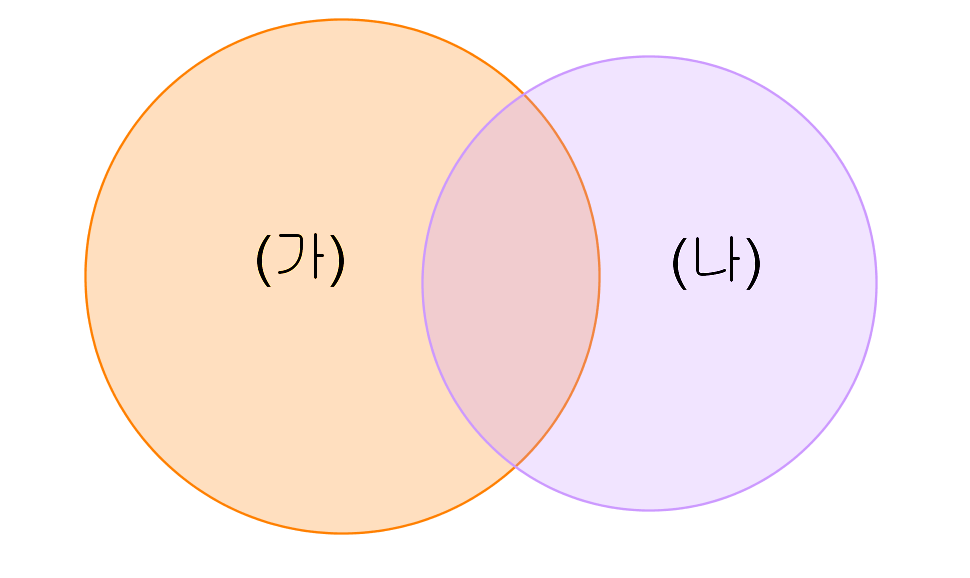
\includegraphics[width=0.5\textwidth]{venn}
\end{figure}
\begin{mdframed}
\textbf{풀이 : }
\vspace{0.15\textheight}
\end{mdframed}

%
\prob
(가) : (나)를 가장 간단한 자연수의 비로 나타내고 그 풀이과정을 쓰세요.
\[
\ga\times\frac38=\na\times0.7
\]
\begin{mdframed}
\textbf{풀이 : }
\vspace{0.15\textheight}
\end{mdframed}
\ans

%
\prob
다음 \(\square\), \(\triangle\)에 들어갈 알맞은 숫자를 구하고 풀이과정을 적으세요.
\[3:6:5=51:\square:\triangle\]
\begin{mdframed}
\textbf{풀이 : }
\vspace{0.15\textheight}
\end{mdframed}


%
\prob
준수와 혜리와 윤주가 색연필 72자루를 2:3:4로 나누어 가지려고 합니다.
준수와 혜리와 윤주가 가지게 되는 색연필은 각각 몇 자루입니까?

{\raggedleft\textbf{
답 :
준수 (\qquad\qquad\qquad\qquad)\\
혜리 (\qquad\qquad\qquad\qquad)\\
윤주 (\qquad\qquad\qquad\qquad)\\
}
\par}\bigskip\bigskip

%
\prob
경민이가 가진 지우개, 연필, 자의 길이의 비는 3:7:8입니다.
연필의 길이가 10.8cm일 때, 지우개와 자의 길이의 합을 구하세요.

\ans

\newpage

%
\prob
가로, 세로, 높이의 비가 2:3:6인 직육면체가 있습니다.
이 직육면체의 모서리의 길이의 합이 121cm일 때, 이 직육면체의 부피를 구하세요.
\begin{figure}[h!]
\centering
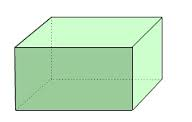
\includegraphics{parallelopipedon}
\end{figure}

\ans


%
\prob
(가)의 0.4는 (나)의 \(\displaystyle\frac37\)과 같을 때 (가) : (나)를 가장 간단한 자연수의 비로 나타내세요.
\begin{figure}[h]
\centering
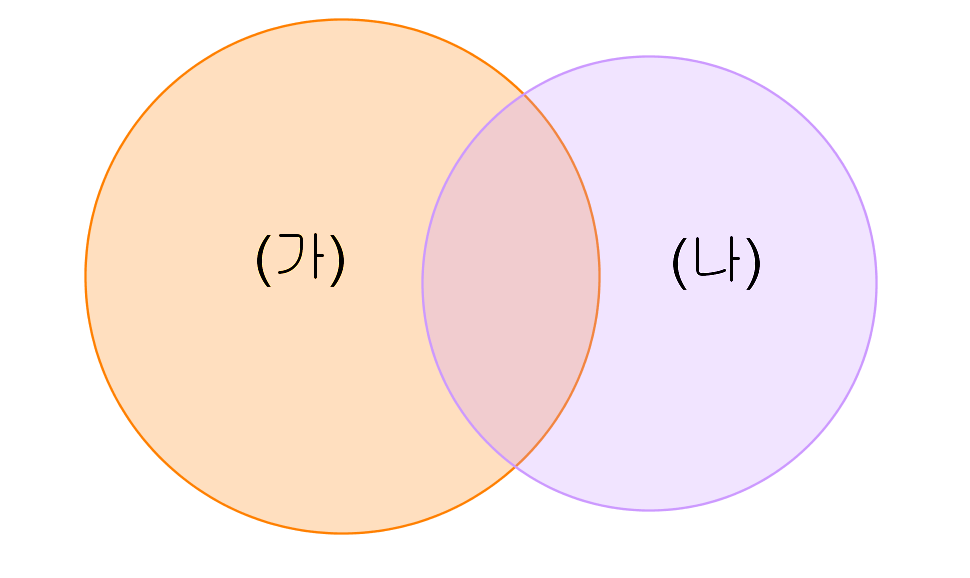
\includegraphics[width=0.5\textwidth]{venn}
\end{figure}

\ans

\newpage
%
\prob
지호와 영신이는 사과 두 개를 먹었습니다.
지호와 영신이가 먹은 사과의 양을 가장 간단한 자연수의 비로 나타내세요.

\ans

\begin{figure}[h!]
\centering
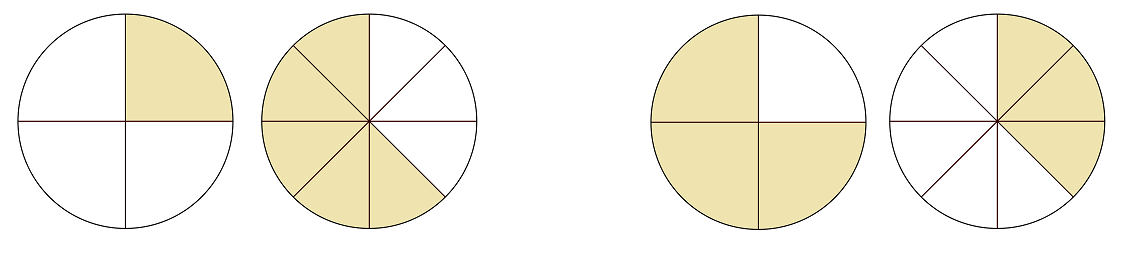
\includegraphics[width=0.9\textwidth]{020}

지호가 먹은 사과\qquad\qquad\qquad\qquad\quad 영신이가 먹은 사과
\end{figure}

%
\prob
지수와 효정이는 사과 두 개를 먹었습니다.
지수와 효정이가 먹은 사과의 양을 가장 간단한 자연수의 비로 나타내세요.

\ans

\begin{figure}[h!]
\centering
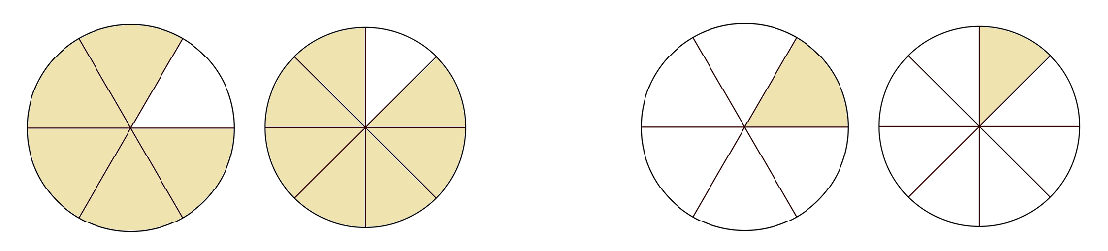
\includegraphics[width=0.9\textwidth]{030}

지수가 먹은 사과\qquad\qquad\qquad\qquad\quad 효정이가 먹은 사과
\end{figure}


%
\prob
다음 \(\square\)에 들어갈 알맞은 숫자를 쓰세요.

\begin{enumerate}[(1)]
\item
\(3:1=\square:\frac37\)
\item
\(3:\frac35=8:\square\)
\item
\(\frac43:\frac32=2:\square\)
\item
\(\frac12:2=3:\square\)
\item
\(1:\frac73=\frac34:\square\)
\item
\(\frac35:\frac45=\square:10\)
\item
\(\frac{12}3:\frac{16}2=\square:\frac{25}2\)
\item
\(\frac{10}7:\frac{25}{11}=\square:28\)
\item
\(\frac{11}2:132=\square:2\)
\item
\(\frac{12}7:5=\frac{6}7:\square\)
\item
\(1.44:1.32=\square:33\)
\item
\(400:650=16:\square\)
\item
\(135:625=0.9:\square\)
\end{enumerate}

\newpage


\end{document}